%%%%%%%%%%%%%%%%%%%%%%%%%%%%%%%%%%%%%%%%%
% Beamer Presentation
% LaTeX Template
% Version 1.0 (10/11/12)
%
% This template has been downloaded from:
% http://www.LaTeXTemplates.com
%
% License:
% CC BY-NC-SA 3.0 (http://creativecommons.org/licenses/by-nc-sa/3.0/)
%
%%%%%%%%%%%%%%%%%%%%%%%%%%%%%%%%%%%%%%%%%

%----------------------------------------------------------------------------------------
%	PACKAGES AND THEMES
%----------------------------------------------------------------------------------------

%\documentclass[handout]{beamer}
\documentclass{beamer}

\mode<presentation> {

% The Beamer class comes with a number of default slide themes
% which change the colors and layouts of slides. Below this is a list
% of all the themes, uncomment each in turn to see what they look like.

%\usetheme{default}
\usetheme{AnnArbor}
%\usetheme{Antibes}
%\usetheme{Bergen}
%\usetheme{Berkeley}
%\usetheme{Berlin}
%\usetheme{Boadilla}
%\usetheme{CambridgeUS}
%\usetheme{Copenhagen}
%\usetheme{Darmstadt}
%\usetheme{Dresden}
%\usetheme{Frankfurt}
%\usetheme{Goettingen}
%\usetheme{Hannover}
%\usetheme{Ilmenau}
%\usetheme{JuanLesPins}
%\usetheme{Luebeck}
%\usetheme{Madrid}
%\usetheme{Malmoe}
%\usetheme{Marburg}
%\usetheme{Montpellier}
%\usetheme{PaloAlto}
%\usetheme{Pittsburgh}
%\usetheme{Rochester}
%\usetheme{Singapore}
%\usetheme{Szeged}
%\usetheme{Warsaw}

% As well as themes, the Beamer class has a number of color themes
% for any slide theme. Uncomment each of these in turn to see how it
% changes the colors of your current slide theme.

%\usecolortheme{albatross}
%\usecolortheme{beaver}
%\usecolortheme{beetle}
%\usecolortheme{crane}
%\usecolortheme{dolphin}
%\usecolortheme{dove}
%\usecolortheme{fly}
%\usecolortheme{lily}
\usecolortheme{orchid}
%\usecolortheme{rose}
%\usecolortheme{seagull}
%\usecolortheme{seahorse}
%\usecolortheme{whale}
%\usecolortheme{wolverine}

%\setbeamertemplate{footline} % To remove the footer line in all slides uncomment this line
%\setbeamertemplate{footline}[page number] % To replace the footer line in all slides with a simple slide count uncomment this line

\setbeamertemplate{navigation symbols}{} % To remove the navigation symbols from the bottom of all slides uncomment this line
}

\usepackage{graphicx} % Allows including images
\usepackage{booktabs} % Allows the use of \toprule, \midrule and \bottomrule in tables
\usepackage[english]{babel}
\usepackage[utf8]{inputenc}
\usepackage{amsmath,amssymb,amsfonts}
\usepackage{times}
\usepackage{fancyvrb}
\usepackage{array}
\usepackage{colortbl}
\usepackage{multirow}
\usepackage{stmaryrd}
\usepackage{booktabs}
\usepackage{calc,xcolor}
\usepackage{url}

\usepackage{tikz}
\usetikzlibrary{positioning,shadows,arrows,shapes,calc,backgrounds,fit}

\usepackage{color,listings}
\definecolor{lightblue}{rgb}{.85,.85,1} % 217 217 255
\definecolor{lightorange}{rgb}{1,.8,.6} % 255 204 153
\definecolor{lightgreen}{rgb}{.6,1,.6} % 153 255 153
\definecolor{lightyellow}{rgb}{1,.98,.6} % 255 250 153
\definecolor{specialblue}{rgb}{.69,.77,.87} % 177 197 222
\definecolor{specialyellow}{rgb}{1.0,.97,.56} % 255 247 143
\definecolor{forestgreen}{RGB}{34,139,34}

\newenvironment<>{newblock}[1]{%
  \begin{actionenv}#2%
      \def\insertblocktitle{#1}%
      \par%
      \mode<presentation>{%
        %\setbeamercolor{block title}{fg=white,bg=darkgray!50}
        \setbeamercolor{block body}{fg=black,bg=white}
       %\setbeamercolor{itemize item}{fg=orange!20!black}
       %\setbeamertemplate{itemize item}[triangle]
     }%
      \usebeamertemplate{block begin}}
    {\par\usebeamertemplate{block end}\end{actionenv}}


%----------------------------------------------------------------------------------------
%	TITLE PAGE
%----------------------------------------------------------------------------------------

\title[Approximate Algorithmic Image Matching]{Approximate Algorithmic Image Matching to Reduce Online Storage Overhead of User Submitted Images} % The short title appears at the bottom of every slide, the full title is only on the title page

%\author[Licastro]{\hspace*{-1.5mm}\mbox{\underline{Braden D. Licastro}}}
\author[Licastro]{Braden D. Licastro} % Your name
\institute[AC] % Your institution as it will appear on the bottom of every slide, may be shorthand to save space
{
Allegheny College, USA \\ % Your institution for the title page
\medskip
\textit{licastb@allegheny.edu} % Your email address
}
%\date{\today} % Date, can be changed to a custom date
\date{April 18, 2014}

\titlegraphic{
\vspace*{-.15in}

\begin{center}

\includegraphics[width=.6\textwidth]{logo_right.pdf}
\end{center}

}

\begin{document}

% Page frame not needed since we are making a title slide.
%\begin{frame}
\frame[plain]{\titlepage} % Print the title page as the first slide with no frame
%\end{frame}

% Fix the page count after the title page.
%\setcounter{tocdepth}{1}

%\begin{frame}
%\frametitle{Overview} % Table of contents slide, comment this block out to remove it
%\tableofcontents % Throughout your presentation, if you choose to use \section{} and \subsection{} commands, these will automatically be printed on this slide as an overview of your presentation
%\end{frame}

%----------------------------------------------------------------------------------------
%	PRESENTATION SLIDES
%----------------------------------------------------------------------------------------

%------------------------------------------------
\section{Motivation} % Sections can be created in order to organize your presentation into discrete blocks, all sections and subsections are automatically printed in the table of contents as an overview of the talk
%------------------------------------------------
\subsection{Re-Introduction}

\begin{frame}
\frametitle{Photo Sharing Service}
\begin{newblock}{Definition}
Photo sharing is the publishing or transfer of a user's digital photos online, thus enabling the user to share them with others \cite{dic:com}.
\end{newblock}
\begin{newblock}{Example Services}
\centering

\includegraphics[width=.2\textwidth]{imgur}

\includegraphics[width=.2\textwidth]{shutterfly}

\includegraphics[width=.2\textwidth]{flickr}

\includegraphics[width=.2\textwidth]{instagram}
\end{newblock}
\end{frame}

%------------------------------------------------
\subsection{Scope of Topic}

\begin{frame}
\frametitle{Remembering the Facts}
\begin{itemize} \itemsep1.5em
\item 500 Million images shared daily \cite{meek:500}
\item Daily image shares expected to double in 2014 \cite{meek:500}
\item Approximately 20\% of stored data is duplicate \cite{ntps:staledata}
\item Eliminating duplicates can save roughly \$1.8 million annually at current sharing levels\footnotemark
\end{itemize}
\footnotetext[1]{Assuming 2013 averages of \$.05 per gigabyte and 1MB image size\cite{ntps:staledata}.}
\end{frame}

%------------------------------------------------
\section{Method of Approach}
%------------------------------------------------
\subsection{Goals Revisited}

\begin{frame}
\frametitle{Goals}
\begin{block}{Website Creation}
Created a flexible website framework that was able to imitate an image sharing service.
\end{block}

\begin{block}{The Algorithm}
Employed a series of checks and algorithms to find and eliminate duplicate and near-duplicate images at the time of upload.
\end{block}

\begin{block}{Result Compilation}
Website generates real time directory file count, directory size, and collects time taken per image upload.
\end{block}
\end{frame}

%------------------------------------------------

\begin{frame}
\frametitle{Website Details}
\begin{figure}
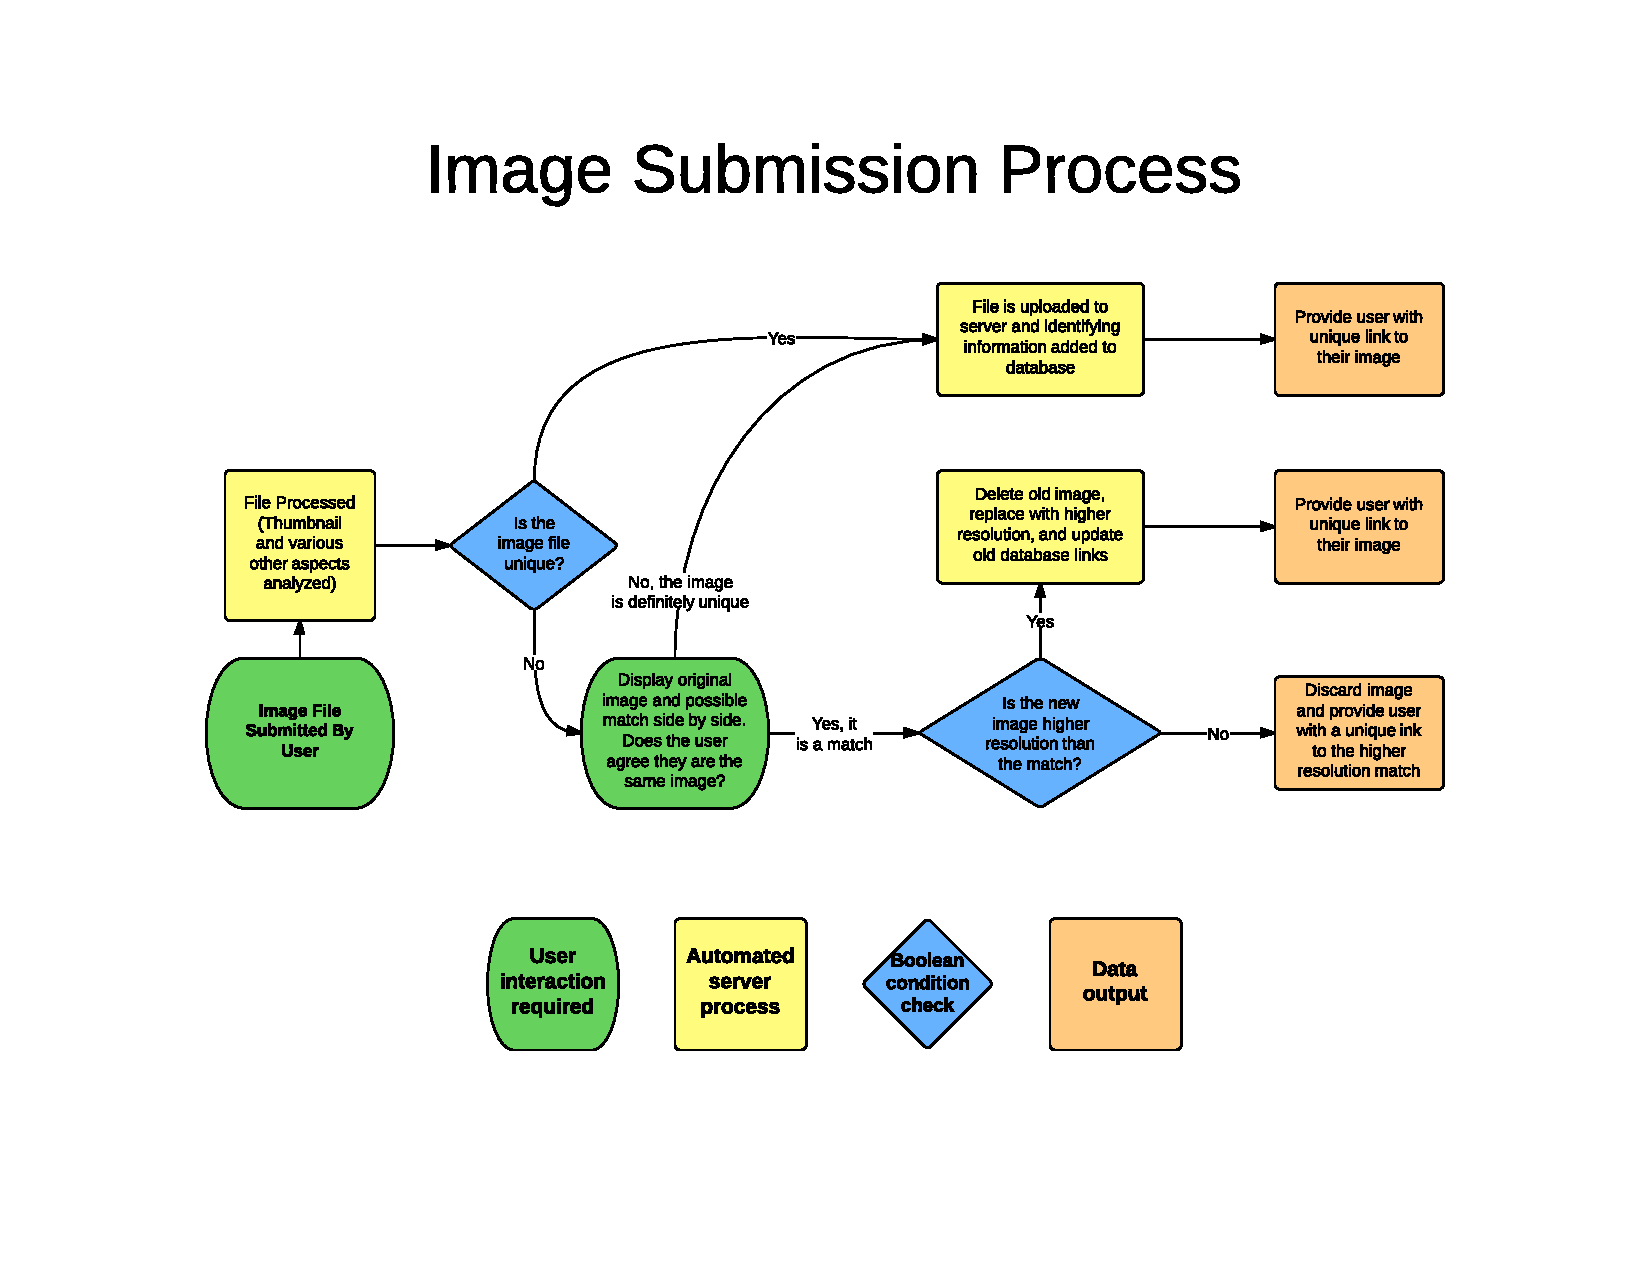
\includegraphics[trim={3cm 3.5cm 2cm 4.2cm},clip, width=.85\textwidth]{upproc}
\caption{Duplicate Identification Process}
\end{figure}
\end{frame}

%------------------------------------------------

\begin{frame}
\frametitle{Website Details}
\begin{figure}
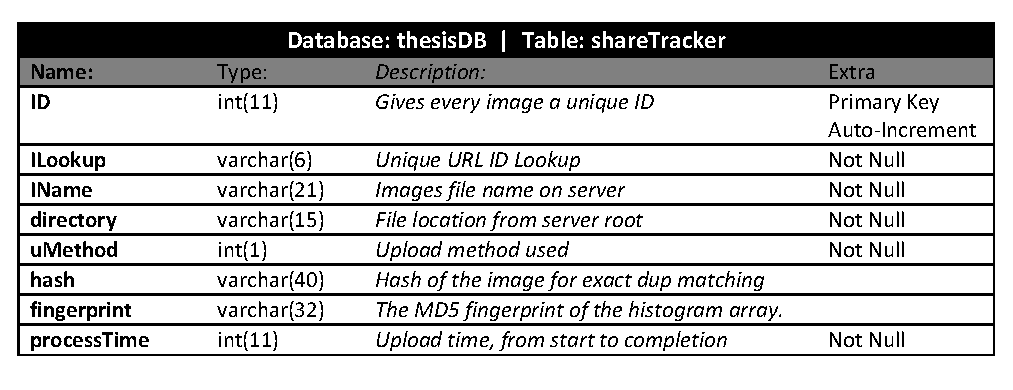
\includegraphics[width=4in]{schema}
\caption{Schema for File Uploads}
\end{figure}
\end{frame}

%------------------------------------------------
\section{Evaluation}
%------------------------------------------------

\subsection{Observed Results} % A subsection can be created just before a set of slides with a common theme to further break down your presentation into chunks

\begin{frame}
\frametitle{Generation of Comparison Data}
\begin{itemize} \itemsep1.5em
\item{Every upload added to baseline directory}
\item{Only unique images added in duplicate-reduced directory}
\item{Time taken for each upload is recorded in the database}
\item{Real time directory statistics updated on every page load}
\end{itemize}
\end{frame}

%------------------------------------------------

\begin{frame}
\frametitle{Test Cases}
\begin{center}
All cases are composed of half computer-\\generated, half photographic imagery.\\

\begin{enumerate}[I] \itemsep1.5em
\item{: Small Images \(<1MB\); No Duplicates}
\item{: Small Images \(<1MB\); 20\% Duplicates}
\item{: Large Images \(>10MB\); No Duplicates}
\item{: Large Images \(>10MB\); 20\% Duplicates}
\end{enumerate}
\end{center}
\end{frame}

%------------------------------------------------

\begin{frame}
\frametitle{Performance Calculation}
\begin{center}
Using this equation, processing time, directory counts,\\and directory size were calculated.
\end{center}
\begin{figure}
\begin{equation} \nonumber
\left ( \frac{Base - Reduced}{Base} \right ) * 100 = \% Improvement Over Base
\end{equation}
\caption{Percent efficiency over base case.}
\end{figure}
\end{frame}

%------------------------------------------------

\begin{frame}
\frametitle{Processing Time}
\begin{center}
Additional processing time minimal given a combined \\unique and duplicate image set.
\end{center}
\begin{figure}
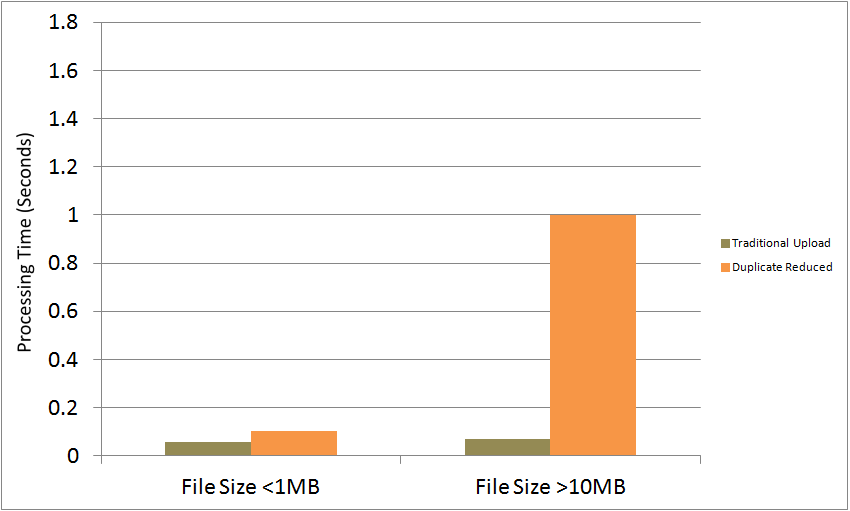
\includegraphics[width=3.25in]{proctimemixdup}
\caption{Processing time on data set with 20\% duplicate images.}
\end{figure}
\end{frame}

%------------------------------------------------

\begin{frame}
\frametitle{Processing Time}
\begin{center}
Worst case processing time is less than twice the previously observed.
\end{center}
\begin{figure}
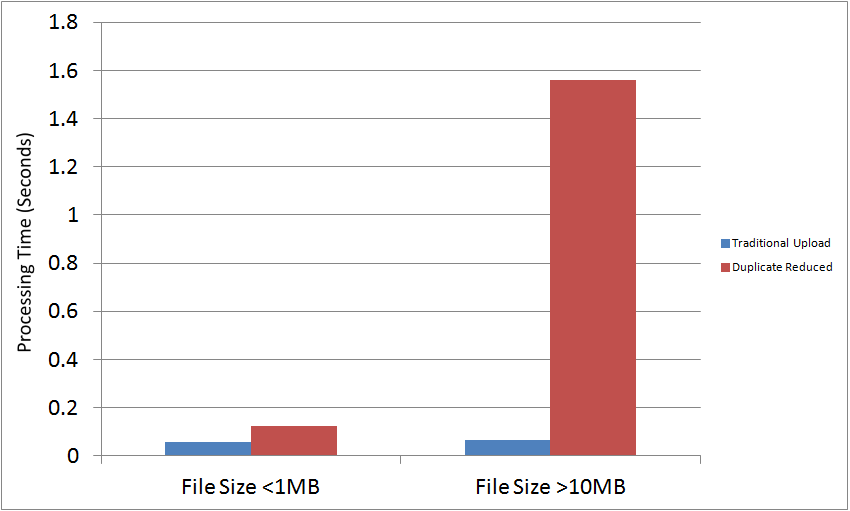
\includegraphics[width=3.25in]{proctimenodup}
\caption{Processing time on data set with no duplicate images.}
\end{figure}
\end{frame}

%------------------------------------------------

\begin{frame}
\frametitle{Storage Requirements}
\begin{center}
After running tests using an average of 20\% duplicate image data...

\textbf{Storage space was reduced approximately 12\%.}
\end{center}
\end{frame}

%------------------------------------------------

\begin{frame}
\frametitle{Detection Rates}
\textbf{Identification patterns led to surprising conclusions:}
\begin{itemize}
\item Correct identification of 82 of 100 small photographs.
\item Identification of 91 of 100 large sized photographs.
\item Surprisingly, only identified 33 of 100 computer generated graphics.
\end{itemize}
\end{frame}

%------------------------------------------------
\section{Exploration of Inconsistencies} % Sections can be created in order to organize your presentation into discrete blocks, all sections and subsections are automatically printed in the table of contents as an overview of the talk
%------------------------------------------------
\subsection{False Positives}

%------------------------------------------------

\begin{frame}
\frametitle{Identification Fault Explored}
\textbf{Low identification numbers were caused by the following:}
\begin{itemize}
\item Large difference in image resolutions.
\item 50/50 black and white distribution of coloring.
\item Small thumbnail size.
\item High detail repetitive patterns.
\end{itemize}
\end{frame}

%------------------------------------------------

\begin{frame}
\frametitle{Dimension and Color Profiles}
\textbf{Resolution causing poor detection:}
\begin{itemize}
\item Reducing image size causes data loss. This is greater in larger images leading to poor detection rates and false positives.
\end{itemize}

\textbf{Color profiles and deep scans:}
\begin{itemize}
\item Black and white images create frequent opportunity for identical color profiles.
\item Matching color profiles require further investigation and re-sizing leading to above problem.
\end{itemize}
\end{frame}

%------------------------------------------------

\begin{frame}
\frametitle{Further Details on Data Loss}
\textbf{Data loss through re-sizing:}
\begin{itemize}
\item Reducing image size averages neighboring pixels into one destination pixel.
\item Fine details will be lost in this process, possibly entirely.
\item Thumbnail analyzed may show false positives  due to this.
\item More prevalent with black and white repetitive patterns.
\end{itemize}

\end{frame}

%------------------------------------------------
\begin{frame}
\frametitle{Data Loss Visualized}
\begin{figure}
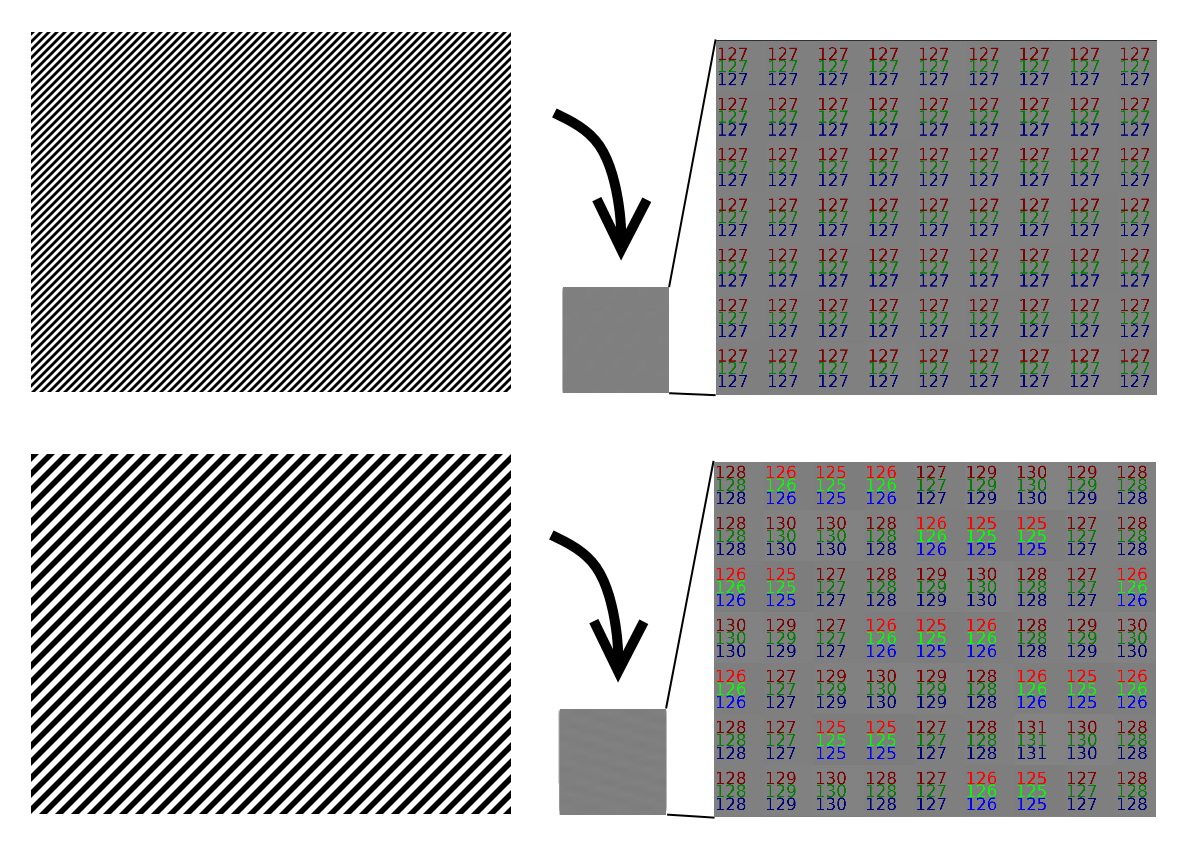
\includegraphics[width=3.25in]{dataloss}
\caption{Visualized data loss after thumbnail creation of pattern.}
\end{figure}

\end{frame}

%------------------------------------------------
\section{Conclusions} % Sections can be created in order to organize your presentation into discrete blocks, all sections and subsections are automatically printed in the table of contents as an overview of the talk
%------------------------------------------------
\subsection{Threats to Validity}

%------------------------------------------------

\begin{frame}
\frametitle{Threats to Validity}
\textbf{Possible areas of concern needing addressed:}
\begin{itemize}
\item Publicly accessible system introduces security vulnerability.
\item Highly specific image modifications tested and may introduce bias.
\item Image corruption possible.
\end{itemize}
\end{frame}

%------------------------------------------------
\subsection{Future Work}

%------------------------------------------------

\begin{frame}
\frametitle{Future Work}
\textbf{Recommended areas of future exploration include:}
\begin{itemize}
\item Expansion of file support allowing for bmp, png, gif, etc.
\item Further optimization of detection accuracy.
\item Allow for other image manipulations.
\item Additional testing, possibly live run for real world data.
\item Determine frequency of hash collisions and impact on results.

\end{itemize}
\end{frame}

%------------------------------------------------

\begin{frame}
\frametitle{Demonstration of Results}
\centering
\Large{View the live website...\\
\href{http://skynetgds.no-ip.biz/srthesis/irc.php}{\beamergotobutton{System Login}}}
\end{frame}

%------------------------------------------------
\section{Conclusion}
%------------------------------------------------

\begin{frame}
\frametitle{References}
\begin{tiny}
\bibliographystyle{plain}
\bibliography{thesis_defense}
\end{tiny}
\end{frame}

%------------------------------------------------

\begin{frame}
\Huge{\centerline{Questions? Comments?}}
\end{frame}

%----------------------------------------------------------------------------------------

\end{document} 